Classic Q-switching question.
\begin{parts}
	\part Q-switching is a technique by which the quality factor of a laser cavity is periodically varied to intentionally build up population inversion $N^*$ beyond the equilibrium value, thus producing a laser output with \textit{large peak intensity} and \textit{short pulse length}.
	
	Q-switching may be achieved by employing a saturable absorber at the output coupler.
	As the absorption of the absorber varies with the intensity $I$, it is able to suppress lasing until saturation, thereby achieving Q-switching without active clock source.
	
	\part
	\begin{subparts}
		\subpart $N^*_\textnormal{th}$ represents the threshold population inversion -- this is the value of $N^*$ when photon population in the cavity begins to grow.
		
		\subpart \textit{Bookwork from Simon's notes.
			Essential points:
			\begin{enumerate}
				\item Integrate $\dderi{n}{t}$ to get relationship between $\dfrac{n}{\tau_c}$'s
				\item Write output power as function of $\dfrac{n}{\tau_c}$ by considering the net photon output rate
				\item ??? {\tiny You know what to do, integration!}
				\item Profit!
			\end{enumerate}
			In any case, I shall demonstrate a (hopefully!) standard answer below.
		}
		
		We integrate $\dderi{n}{t}$ as given in the question:
		\begin{align*}
			\defint{n(t\rightarrow-\infty)}{n(t\rightarrow+\infty)}{}{n} &= \defint{-\infty}{+\infty}{}{t} \, \rbracket{\frac{N^*}{N^*_\textnormal{th}} - 1}\frac{n}{\tau_c} \\
			\Rightarrow \underbracket{n(t\rightarrow+\infty) - n(t\rightarrow-\infty)}_\textnormal{0 since we have null intensity in either limit!} &= \ldots \\
			\Rightarrow \defint{-\infty}{+\infty}{}{t} \, \frac{n}{\tau_c} &= \defint{-\infty}{+\infty}{}{t} \, \frac{N^*}{N^*_\textnormal{th}} \, \frac{n}{\tau_c}
		\end{align*}
		
		Then note that the power output is just (net photon output rate) $\times\,\hbar\omega$:
		\begin{equation}
			P = \rbracket{\frac{nV_c}{\tau_c}}\hbar\omega
			\label{eqn:cavity-output}
		\end{equation}
		Note that the net output photon \textit{(not density!}) rate involves the product with the cavity volume!
		
		Integrating \eqref{eqn:cavity-output} then gives (also noting the given $\dderi{N^*}{t}$):
		\begin{align*}
			E &= \defint{-\infty}{+\infty}{P}{t} \\
			&= \defint{-\infty}{+\infty}{}{t} \, \frac{n}{\tau_c} V_c \hbar\omega \\
			&= \defint{-\infty}{+\infty}{}{t} \, \frac{N^*}{N^*_\textnormal{th}}\, \frac{n}{\tau_c} V_c \hbar\omega \\
			&= \defint{N^*(t \to -\infty)}{N^*(t \to +\infty)}{}{N^*} \, \rbracket{-\frac{f_c}{\beta} V_c \hbar\omega} \\
			&= \frac{N^*_\textnormal{i} - N^*_\textnormal{f}}{\beta} V_g \hbar\omega \\
			&= \eta N^*_\textnormal{i} V_g \hbar\omega
		\end{align*}
		
		\subpart From above, $\eta = \dfrac{N^*_\textnormal{i} - N^*_\textnormal{f}}{\beta N^*_\textnormal{i}}$ is the energy utilisation factor.
		This encodes how efficient the laser system is in extracting energy from population inversion.
	\end{subparts}
	
	\part
	\begin{subparts}
		\subpart To find $n(t)$, we divide $\dderi{n}{t}$ by $\dderi{N^*}{t}$ to get:
		\begin{align*}
			\deri{n}{N^*} &= -\frac{f_c}{\beta} \rbracket{1 - \frac{N^*_\textnormal{th}}{N^*}} \\
			\Rightarrow \defint{N^* (0)}{N^* (t)}{
				\rbracket{1 - \frac{N^*_\textnormal{th}}{N^*}}
			}{N^*} &= \defint{n(0)}{n(t)}{-\frac{\beta}{f_c}}{n} \\
			-\frac{\beta}{f_c} \rbracket{n(t) - n(0)} &= \rbracket{N^* (t) - N^* (0)} - N^*_\textnormal{th} \ln\rbracket{\frac{N^* (t)}{N^*(0)}}
		\end{align*}
		
		Equating $n(0) = 0$ and $N^*(0) = N^*_\textnormal{i}$ gives:
		\begin{equation*}
			n(t) = \frac{f_c}{\beta} \sbracket{ N^*_\textnormal{th}\ln\rbracket{\frac{N^* (t)}{N^*_\textnormal{i}}} + \rbracket{N^*_\textnormal{i} - N^* (t)} }
		\end{equation*}
		
		\subpart Now putting in limits of $n(t\rightarrow+\infty)=0$, $N^* (t\rightarrow+\infty)=N^*_\textnormal{f}$:
		\begin{align*}
			N^*_\textnormal{f} - N^*_\textnormal{i} &= N^*_\textnormal{th} \ln\rbracket{\frac{N^*_\textnormal{f}}{N^*_\textnormal{i}}} \\
			\Rightarrow \beta\eta N^*_\textnormal{i} &= N^*_\textnormal{th} \ln\rbracket{\frac{N^*_\textnormal{i}}{N^*_\textnormal{i}\rbracket{1 - \beta\eta}}} \\
			\beta\eta &= \frac{1}{r} \ln\rbracket{\frac{1}{1 - \beta\eta}} \\
			r &= - \frac{\ln\rbracket{1-\beta\eta}}{\beta\eta}
		\end{align*}
		\newpage
		\subpart \textit{Precise sketch may be found in Simon's notes:}
		\begin{figure}[H]
			\centering
			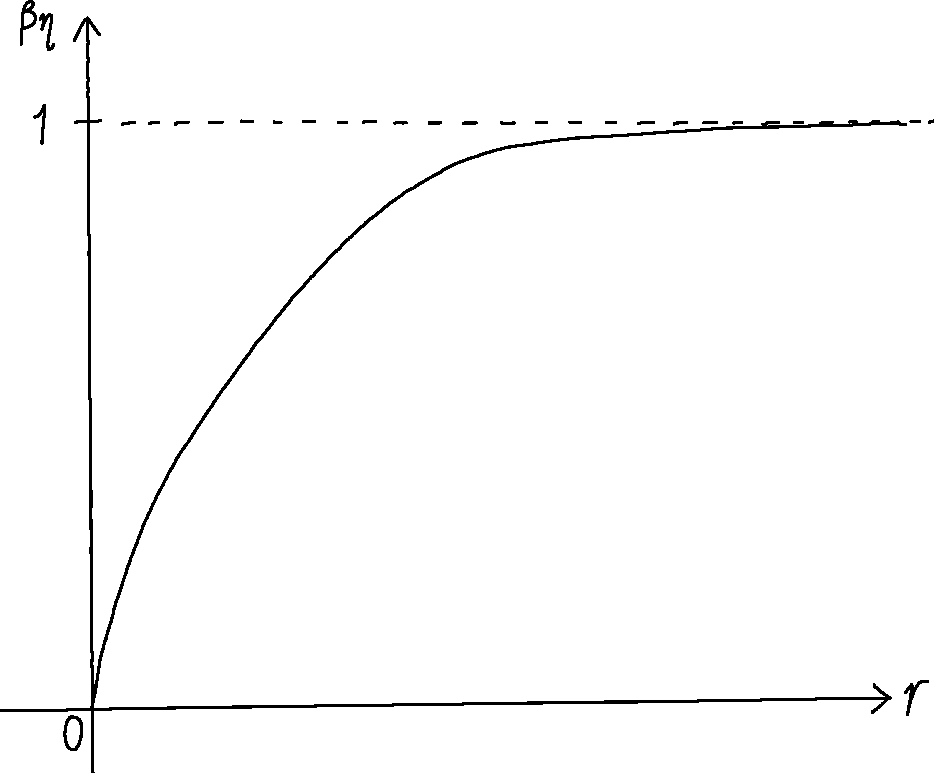
\includegraphics[width=.7\linewidth]{q1-betaeta-r}
		\end{figure}
		
		\subpart For $E / E_\textnormal{max} = \SI{95}{\percent}$, we have:
		\begin{align*}
			\beta&\eta = 0.95 \\
			\Rightarrow r &= - \frac{\ln 0.05}{0.95} \\
			&= 3.15
		\end{align*}
	\end{subparts}
	
	\part Setting $\dderi{n}{t} = 0$ gives $N^* = N^*_\textnormal{th}$.
	substituting this into $n(t)$ then gives:
	\begin{align*}
		n_\textnormal{peak} &= \frac{f_c}{\beta} \sbracket{ N^*_\textnormal{th}\ln\rbracket{\frac{N^*_\textnormal{th}}{N^*_\textnormal{i}}} + \rbracket{N^*_\textnormal{i} - N^*_\textnormal{th})} } \\
		&= \frac{f_c}{\beta} N^*_\textnormal{i} \sbracket{ \frac{1}{r} \ln\rbracket{\frac{1}{r}} + \rbracket{1 - \frac{1}{r}} }
	\end{align*}
	
	Substituting this into \eqref{eqn:cavity-output} then gives the peak power:
	\begin{align}
		P_\textnormal{peak} &= \frac{N^*_\textnormal{i} f_c V_c \hbar\omega}{\beta\tau_c} \sbracket{ \frac{-\ln r + r - 1}{r} } \notag \\
		&= \frac{N^*_\textnormal{i} V_g \hbar\omega}{\beta\tau_c} \sbracket{ \frac{r-1-\ln r}{r} } \label{eqn:peak-power}
	\end{align}
	
	Rewriting \eqref{eqn:peak-power} in terms of $N^*_\textnormal{th}$:
	\begin{align*}
		P_\textnormal{peak} &= \frac{N^*_\textnormal{i} f_c V_c \hbar\omega}{\beta\tau_c} \sbracket{ \frac{-\ln r + r - 1}{r} } \notag \\
		&= \frac{N^*_\textnormal{th} V_g \hbar\omega}{\beta\tau_c} \sbracket{ r-1-\ln r }
	\end{align*}
	
	At large $r$, the peak output power grows towards $\infty$ as the laser system is able to burn almost all of the population inversion down to generate an intense pulse.
	
	As suggested by the rate equations above, large value of $r$ will also cause a rapid population burning, hence the pulse will possess a short pulse length as shown in the sketch below:
	\begin{figure}[H]
		\centering
		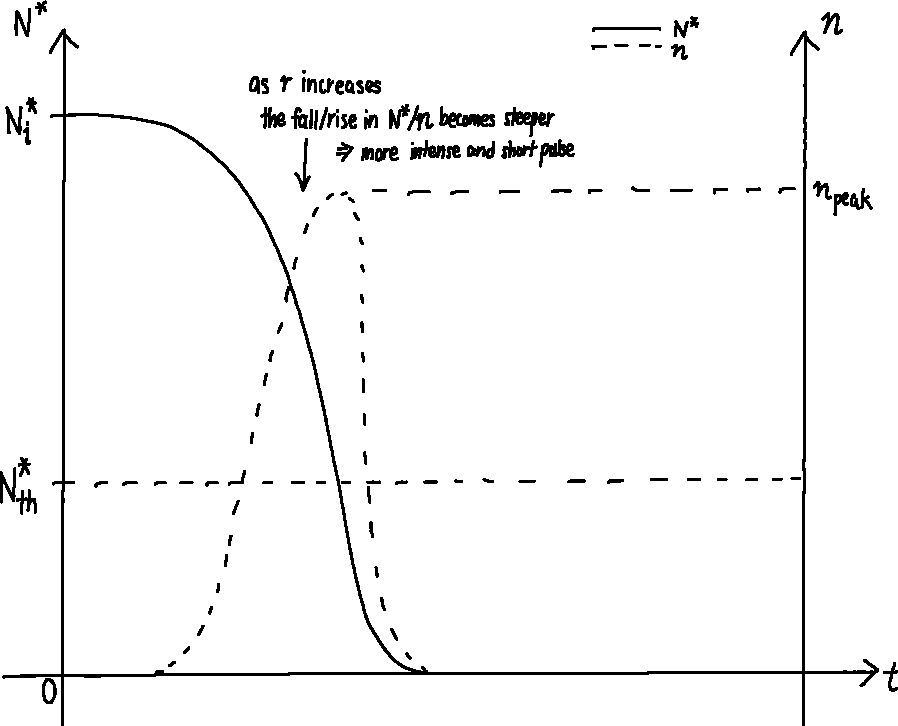
\includegraphics[width=.8\linewidth]{q1-pulse-profile}
	\end{figure}
\end{parts}